% Options for packages loaded elsewhere
\PassOptionsToPackage{unicode}{hyperref}
\PassOptionsToPackage{hyphens}{url}
\documentclass[
]{article}
\usepackage{xcolor}
\usepackage{amsmath,amssymb}
\setcounter{secnumdepth}{-\maxdimen} % remove section numbering
\usepackage{iftex}
\ifPDFTeX
  \usepackage[T1]{fontenc}
  \usepackage[utf8]{inputenc}
  \usepackage{textcomp} % provide euro and other symbols
\else % if luatex or xetex
  \usepackage{unicode-math} % this also loads fontspec
  \defaultfontfeatures{Scale=MatchLowercase}
  \defaultfontfeatures[\rmfamily]{Ligatures=TeX,Scale=1}
\fi
\usepackage{lmodern}
\ifPDFTeX\else
  % xetex/luatex font selection
\fi
% Use upquote if available, for straight quotes in verbatim environments
\IfFileExists{upquote.sty}{\usepackage{upquote}}{}
\IfFileExists{microtype.sty}{% use microtype if available
  \usepackage[]{microtype}
  \UseMicrotypeSet[protrusion]{basicmath} % disable protrusion for tt fonts
}{}
\makeatletter
\@ifundefined{KOMAClassName}{% if non-KOMA class
  \IfFileExists{parskip.sty}{%
    \usepackage{parskip}
  }{% else
    \setlength{\parindent}{0pt}
    \setlength{\parskip}{6pt plus 2pt minus 1pt}}
}{% if KOMA class
  \KOMAoptions{parskip=half}}
\makeatother
\usepackage{graphicx}
\makeatletter
\newsavebox\pandoc@box
\newcommand*\pandocbounded[1]{% scales image to fit in text height/width
  \sbox\pandoc@box{#1}%
  \Gscale@div\@tempa{\textheight}{\dimexpr\ht\pandoc@box+\dp\pandoc@box\relax}%
  \Gscale@div\@tempb{\linewidth}{\wd\pandoc@box}%
  \ifdim\@tempb\p@<\@tempa\p@\let\@tempa\@tempb\fi% select the smaller of both
  \ifdim\@tempa\p@<\p@\scalebox{\@tempa}{\usebox\pandoc@box}%
  \else\usebox{\pandoc@box}%
  \fi%
}
% Set default figure placement to htbp
\def\fps@figure{htbp}
\makeatother
\setlength{\emergencystretch}{3em} % prevent overfull lines
\providecommand{\tightlist}{%
  \setlength{\itemsep}{0pt}\setlength{\parskip}{0pt}}
\usepackage{bookmark}
\IfFileExists{xurl.sty}{\usepackage{xurl}}{} % add URL line breaks if available
\urlstyle{same}
\hypersetup{
  hidelinks,
  pdfcreator={LaTeX via pandoc}}

\author{}
\date{}

\begin{document}

\section{The Floating Neutral: Endogenous Reference Theory and Moral
Reference Without
Authority}\label{the-floating-neutral-endogenous-reference-theory-and-moral-reference-without-authority}

\textbf{Andrew H. Bond} San José State University · andrew.bond@sjsu.edu
· ORCID 0009-0003-2599-6158

\emph{Draft v0.1 --- a metaethical companion to the Geometric Ethics
program. Status: working paper.}

\begin{center}\rule{0.5\linewidth}{0.5pt}\end{center}

\subsection{Abstract}\label{abstract}

Metaethical realism and anti-realism share an unexamined assumption:
that a moral \emph{reference} --- the standard against which actions are
judged --- requires an \emph{anchor}. The realist seeks the anchor in
mind-independent binding facts (or in God); the anti-realist, finding no
such anchor, concludes there is no determinate moral fact at all, only
projection, error, or arbitrary commitment. We reject the shared
assumption. Drawing on the behavior of a \textbf{floating neutral} in a
polyphase electrical system, we develop \textbf{Endogenous Reference
Theory (ERT)}: the moral reference of a system is a determinate,
computable point fixed entirely by the system's own constituents --- its
agents and their weighted valuations --- with no external anchor and
\emph{no normative authority}. The reference has a \emph{location} but
issues no \emph{commands}. On this view ``ought'' does not name a
binding force transmitted from a higher level; it names
\textbf{displacement} from the endogenous reference --- a strain, not a
decree. ERT makes three contributions the existing literature lacks: (i)
a \emph{determinate yet anchorless} referent, given a closed-form
construction (the load-weighted Fréchet mean on a moral manifold, the
geometric generalization of Millman's theorem); (ii) a \textbf{reflexive
control dynamics} in which agents re-weight their own valuations and
thereby move the reference they are measured against, recasting moral
change as feedback rather than convergence toward a fixed target; and
(iii) a \emph{dissolution} rather than a solution of the is/ought
problem --- the far bank of Hume's gap is shown to be a mirage of the
anchoring assumption. ERT is deflationary about authority and realist
about structure. It is also falsifiable, and we state the conditions
that would refute it.

\begin{center}\rule{0.5\linewidth}{0.5pt}\end{center}

\subsection{1. The shared assumption}\label{the-shared-assumption}

Ask what makes an action good and two answers dominate. The
\textbf{realist} says: there is a fact of the matter, binding
independently of what anyone thinks --- perhaps grounded in the nature
of reasons, perhaps in God. The \textbf{anti-realist} says: there is no
such fact; ``good'' expresses an attitude, encodes an error, or marks an
arbitrary brute commitment that bottoms out a regress (one cannot rank
two values without appealing to a third, \emph{ad infinitum}).

These positions look opposed, but they agree on something deeper. Both
assume that for a moral reference to be \emph{real} --- determinate,
non-arbitrary, action-guiding --- it must be \textbf{anchored} to
something outside the system of valuers: a transcendent ground, a
Platonic fact, a divine will. The realist affirms the anchor; the
anti-realist, having looked and found none, infers that the reference
itself is empty. The dilemma --- \emph{binding external fact, or
arbitrary brute} --- is generated by the anchoring assumption, not by
morality.

This paper denies the assumption. We claim that a moral reference can be
\textbf{determinate without being anchored}, and that the model for such
a thing is already familiar to any electrical engineer.

\textbf{A note on method.} ERT is offered in the spirit of
\emph{Philosophy Engineering}: the discipline of stating a philosophical
claim formally enough that it can be computed, made to predict, and
broken. Where traditional metaethics argues toward a position and rests,
ERT is built to be \emph{operated} --- it gives the moral reference a
closed-form construction (the load-weighted Fréchet mean, §3), derives
consequences that could have come out otherwise (the conservation law,
§5.2; the schism threshold, §5.6), exposes a falsification battery (§8),
and ships with a reproducible computational artifact that both verifies
the formal results numerically and applies them to real moral-judgment
data --- continuing the program of the Geometric Ethics framework
{[}Bond 2026{]}. A metaethics that cannot be wrong in public is, on this
view, not yet finished; the rest of this paper is an attempt to make ERT
wrong and a report of where it survives.

\subsection{2. The model: a floating
neutral}\label{the-model-a-floating-neutral}

In a polyphase power system, several live conductors (the \emph{phases})
drive a set of loads that meet at a common point, the \emph{neutral}.
When the neutral is \emph{bonded} --- tied to an external ground --- its
potential is clamped to zero; it has an anchor, and the phase voltages
are measured against it.

Remove the bond. The neutral now \textbf{floats}. One might expect it to
become undefined, or to wander arbitrarily. It does neither. The
floating neutral sits at a perfectly definite potential, given by
\textbf{Millman's theorem} {[}Millman 1940{]}:

\[ V_N \;=\; \frac{\sum_i Y_i\,V_i}{\sum_i Y_i}, \qquad Y_i = 1/Z_i, \]

the \textbf{admittance-weighted average} of the phase voltages \(V_i\),
where \(Y_i\) is the load on phase \(i\). No external reference appears
anywhere in this expression. The neutral's location is fixed
\emph{entirely by the loads} --- by the system's own internal
configuration. It is determinate, measurable, and computable; it is also
anchorless. Shift the loads and it moves; balance them and it centers;
lose a load and it lurches. It is a real point with no ground beneath
it.

Two facts about the floating neutral do the philosophical work.

\textbf{First: it has a position but no authority.} The neutral does not
\emph{command} the phases; it is simply where they net out. A phase is
under no obligation to ``honor'' the neutral. Yet the neutral is not
inert: a badly displaced neutral --- under a severe load imbalance ---
drives overvoltages that \emph{destroy equipment}. It has consequences
without commands. Position, not authority.

\textbf{Second: it is endogenous.} Ask ``what grounds the neutral's
location?'' and the only honest answer is \emph{nothing external grounds
it; it is constituted by the loads.} Asking what \emph{authorizes} it is
a category error, like asking what authorizes the center of mass of a
galaxy.

ERT is the claim that \textbf{moral reference is a floating neutral.}

\subsection{3. Endogenous Reference
Theory}\label{endogenous-reference-theory}

Let a moral system comprise agents (or, more abstractly, value-bearing
positions) indexed by \(i\). Each contributes a \emph{valuation} \(v_i\)
--- a position in a moral state space --- held with a \emph{weight}
\(w_i\) (its intensity, prevalence, or ``load''). The system's moral
reference is the endogenous point

\[ R \;=\; \arg\min_{x}\ \sum_i w_i\, d(x, v_i)^2, \]

the \textbf{weighted Fréchet mean} {[}Fréchet 1948{]} of the valuations
under the metric \(d\) of the state space. On a flat space this reduces
exactly to Millman's weighted average {[}Millman 1940{]}; on the curved
\textbf{moral manifold} of Geometric Ethics {[}Bond 2026{]} (a
nine-dimensional stratified space with a context-dependent metric), it
is its geometric generalization. \(R\) is determinate given the loads,
computable, and anchorless: no term outside the set of valuers enters
its definition.

ERT then makes a sequence of claims:

\begin{enumerate}
\def\labelenumi{\arabic{enumi}.}
\tightlist
\item
  \textbf{Realism about the reference.} \(R\) is a real feature of the
  system --- not a projection, not an error, not a fiction. Two analysts
  with the same load data compute the same \(R\). The anti-realist's
  ``no determinate fact'' is false: there is a fact, the location of
  \(R\).
\item
  \textbf{Deflationism about authority.} \(R\) has no normative force.
  It does not bind any agent to itself. The realist's ``binding fact''
  is false: \(R\) commands nothing.
\item
  \textbf{``Ought'' as displacement.} Normative language reports the
  relation of a state to \(R\). ``\(a\) is wrong'' says, roughly,
  \emph{\(a\) lies far from \(R\) along load-bearing dimensions} --- it
  is a \textbf{strain reading}, not a decree. The intensity of moral
  feeling tracks displacement magnitude the way strain voltage tracks
  neutral shift.
\item
  \textbf{Endogeneity.} \(R\) is constituted by the loads. There is no
  meta-level --- no anchor, no transcendent ground, no ``moral law''
  above the system. \emph{There is only the configuration, and the point
  it determines.}
\end{enumerate}

The user's slogan captures it exactly: \emph{there is no bindingness;
there is no meta-anything; there is only reality.} ERT is the formal
content of that slogan.

\subsection{4. The is/ought gap,
dissolved}\label{the-isought-gap-dissolved}

Hume {[}1739{]} observed that one cannot validly derive an \emph{ought}
from an \emph{is}. The realist treats this as a gap to be bridged; the
anti-realist, as a proof that oughts are not facts. ERT treats it as a
\textbf{mislocated demand.}

The gap is the distance between descriptive fact and a \emph{binding}
prescription --- a prescription with authority, transmitted from
somewhere. But on ERT there is no such bank on the far side to reach.
The floating neutral has position, not authority; ``ought'' is the
\emph{strain}, which is itself an is-fact (a displacement is a
measurable quantity). There is no leap from is to ought because
``ought,'' properly understood, was an is all along --- the is of
\emph{displacement from the endogenous reference.}

This is a \emph{dissolution}, and it has a cost we state plainly (§7):
one who uses ``ought'' to mean \emph{categorically binding} will say we
have changed the subject. We have --- deliberately. The categorical bind
was the anchoring assumption's shadow; remove the anchor and the shadow
goes with it. What remains --- real reference, real displacement, real
consequences --- is everything morality needs to \emph{function}, and
nothing it needs to \emph{command}.

\subsection{5. Reflexive dynamics: a
formalization}\label{reflexive-dynamics-a-formalization}

Here ERT departs decisively from a static picture, and from its
electrical metaphor. In a power system a phase cannot choose its own
impedance. \textbf{Agents can.} A valuer can re-weight its own valuation
--- come to care differently --- and thereby move the reference \(R\)
against which it, and everyone else, is measured. The system
\emph{steers itself relative to its own floating point.} We make this
precise.

\subsubsection{5.1 State and reference}\label{state-and-reference}

Let agents be indexed \(i = 1,\dots,N\), each with a valuation
\(v_i \in \mathbb{R}^n\) (a local chart of the moral manifold \(M\)) and
a non-negative weight (load) \(w_i\), with total \(W = \sum_i w_i\). The
endogenous reference is the weighted Fréchet mean {[}Fréchet 1948{]},

\[ R \;=\; \arg\min_x \sum_i w_i\, d(x, v_i)^2, \]

which in the Euclidean case reduces exactly to the Millman point
{[}Millman 1940{]},

\[ R \;=\; \frac{1}{W}\sum_i w_i\, v_i \;=\; \langle v\rangle_w . \]

We work in the flat case for the analytic results and return to the
manifold in §5.5.

\subsubsection{5.2 The law of reference
motion}\label{the-law-of-reference-motion}

Let valuations and weights evolve smoothly in time. Differentiating
\(R = (\sum_i w_i v_i)/W\) gives the central identity

\[ \boxed{\ \dot R \;=\; \underbrace{\langle \dot v\rangle_w}_{\text{position drift}} \;+\; \underbrace{\tfrac{1}{W}\sum_i \dot w_i\,(v_i - R)}_{\text{reweighting}}\ } \qquad(\star) \]

where \(\langle \dot v\rangle_w = \tfrac{1}{W}\sum_i w_i \dot v_i\). The
reference moves by exactly two routes: a net weighted \textbf{drift} of
valuations, or a \textbf{reweighting} that loads one side of the current
reference (a covariance between weight change and displacement). Nothing
external can move it --- consistent with endogeneity.

\textbf{Proposition 1 (Conservation of the reference under homogeneous
conformity).} \emph{If weights are fixed (\(\dot w_i = 0\)) and every
agent relaxes toward the reference at a common rate,
\(\dot v_i = k\,(R - v_i)\) with \(k>0\), then \(\dot R = 0\). The
reference is invariant, and the configuration converges to consensus at
\(R(0)\), with dispersion \(\sum_i w_i \lVert v_i - R\rVert^2\) decaying
as \(e^{-2kt}\).}

\emph{Proof.} By \((\star)\),
\(\dot R = \langle \dot v\rangle_w = \tfrac{1}{W}\sum_i w_i k (R - v_i) = k(R - \langle v\rangle_w) = k(R - R) = 0\).
With \(R\) fixed, \(\tfrac{d}{dt}(v_i - R) = -k(v_i - R)\), so each
displacement decays as \(e^{-kt}\) and the weighted dispersion as
\(e^{-2kt}\). \(\square\)

This has a sharp consequence:

\textbf{Corollary (Progress is not free).} \emph{A purely conformist
population cannot move its own moral reference.} Reference motion
requires an \textbf{asymmetry}: heterogeneous responsiveness, weight
dynamics, nonlinearity, or exogenous forcing. The floating neutral does
not drift on its own; something must load it.

The heterogeneous case makes the mechanism explicit. With
\(\dot v_i = k_i(R - v_i)\) and fixed weights,

\[ \dot R \;=\; \frac{\sum_i w_i k_i}{W}\,\bigl(R - R_k\bigr), \qquad R_k \;=\; \frac{\sum_i w_i k_i\, v_i}{\sum_i w_i k_i}, \]

so the reference drifts \textbf{toward the responsiveness-weighted mean}
\(R_k\) --- i.e., toward the positions of the agents who update fastest
and are weighted most heavily. The neutral is pulled by whoever moves
first and loudest, not by who is ``right.''

\subsubsection{5.3 Regimes}\label{regimes}

Add a \emph{conviction} (differentiation) term that pushes an agent away
from the reference --- identity, contrarianism, principled resistance:

\[ \dot v_i \;=\; \underbrace{k_i\,(R - v_i)}_{\text{conformity}} \;-\; \underbrace{c_i\, \phi(v_i - R)}_{\text{conviction}}, \qquad \dot w_i \;=\; \alpha\, \psi(v_i - R) . \]

The qualitative outcomes mirror those of bounded-confidence opinion
dynamics {[}Hegselmann--Krause 2002{]} --- consensus, polarization, or
fragmentation --- selected by the conformity/conviction balance and the
weight-feedback gain \(\alpha\):

\begin{itemize}
\tightlist
\item
  \textbf{Conformity-dominated} (\(c_i \approx 0\)): consensus at a
  conserved neutral (Prop. 1).
\item
  \textbf{Balanced}: a stable \emph{dispersed} equilibrium ---
  persistent disagreement around a stable reference (a ``moral
  ecology''), not collapse to unanimity.
\item
  \textbf{Conviction- or feedback-dominated}: polarization (bimodal
  split) or \textbf{limit cycles} (moral oscillation), as the
  reweighting term in \((\star)\) drives and is driven by displacement.
\end{itemize}

\textbf{Shocks.} If a faction's load vanishes abruptly, \(w_j \to 0\),
the reference lurches by \(\Delta R \approx -\tfrac{w_j}{W}(v_j - R)\)
--- the neutral jumps away from the departed position, and the remaining
agents experience a sudden jump in their own displacement: the moral
analogue of losing a phase and driving \textbf{overvoltage} on the rest.
This models norm collapse, generational turnover, and revolution as the
\emph{same} mechanism, differing only in rate.

\subsubsection{5.4 Equilibria and
stability}\label{equilibria-and-stability}

A self-consistent equilibrium is a configuration
\(\{v_i^{*}, w_i^{*}\}\) with \(\dot v_i = \dot w_i = 0\) and
\(R = R(\{v_i^{*}, w_i^{*}\})\). The system is
\textbf{self-referential}: each agent's motion feeds back through the
mean, \(\partial R/\partial v_j = w_j/W\), so the Jacobian is not
block-diagonal. The consensus equilibrium (\(v_i = R\), conformity only)
has eigenvalues \(-k_i\) and is asymptotically stable. Dispersed
equilibria are stable when conformity dominates conviction at the fixed
point; crossing that balance produces a Hopf bifurcation into the
oscillatory regime. We state these as the structure of the analysis; the
full classification on \(M\) is open (§5.8).

\subsubsection{5.5 Relation to existing dynamics, and what is actually
new}\label{relation-to-existing-dynamics-and-what-is-actually-new}

Honesty requires naming the neighbors. Equation \((\star)\) and the
regimes of §5.3 are close kin to consensus and opinion-dynamics models
--- DeGroot averaging {[}DeGroot 1974{]}, the Friedkin--Johnsen
extension, and bounded-confidence dynamics {[}Hegselmann--Krause
2002{]}. \textbf{ERT does not claim to invent this mathematics.} Its
contributions over that literature are three, and they are conceptual
before they are technical:

\begin{enumerate}
\def\labelenumi{\arabic{enumi}.}
\tightlist
\item
  \textbf{Interpretation.} The consensus point is reinterpreted as the
  \emph{moral reference} --- the floating neutral --- and ``ought'' as
  displacement from it. The opinion-dynamics literature studies
  \emph{where opinions go}; ERT reads the same object as \emph{the
  metaethical reference itself}, with no anchor and no authority.
\item
  \textbf{Loads as first-class.} Standard models fix influence weights
  or set them exogenously; ERT makes the weight dynamics \(\dot w_i\)
  co-equal with \(\dot v_i\), which is what equation \((\star)\) shows
  is \emph{necessary} for the reference to move at all (the Corollary).
  Reflexive reweighting is the engine of moral change.
\item
  \textbf{Curvature.} Lifting to the moral manifold \(M\), \(R\) is the
  weighted Fréchet/Karcher mean {[}Karcher 1977{]}, whose existence and
  uniqueness require curvature and locality conditions {[}Afsari
  2011{]}. Disagreement spread across a region of high curvature or near
  a cut locus can make \(R\) non-unique --- a genuinely new phenomenon
  with no flat-space or scalar analogue: \emph{the reference can
  bifurcate}, a candidate formal model of moral schism.
\end{enumerate}

The one result we do claim as ERT's own is the \textbf{conservation law
\((\star)\) together with Proposition 1 and its Corollary}, read
metaethically: a self-referencing valuing system cannot move its own
reference without an internal asymmetry. That is a falsifiable,
non-obvious statement about moral change, and it falls directly out of
taking the floating-neutral picture seriously. The second is the schism
result below, which has no scalar or flat-space analogue at all.

\subsubsection{5.6 Schism: bifurcation of the moral
reference}\label{schism-bifurcation-of-the-moral-reference}

The reference \(R\) minimizes the Fréchet function
\(F(x) = \tfrac12\sum_i w_i\, d(x, v_i)^2\). Whether \(R\) is
\emph{unique} is not a metaethical stipulation --- it is a fact about
the \textbf{curvature} of the value space, and it is where ERT makes a
prediction no flat or scalar theory can.

\textbf{The geometry.} For a single datum \(p\), the Hessian of
\(\tfrac12 d(\cdot,p)^2\) on a space of constant sectional curvature
\(\kappa\) has eigenvalue \(1\) along the geodesic toward \(p\) and, in
the orthogonal directions,

\[ h_\kappa(d) \;=\; \sqrt{\kappa}\,d\,\cot\!\bigl(\sqrt{\kappa}\,d\bigr) \quad (\kappa>0), \qquad h_0(d)=1, \qquad h_\kappa(d)=\sqrt{-\kappa}\,d\coth\!\bigl(\sqrt{-\kappa}\,d\bigr)\ (\kappa<0). \]

The Fréchet Hessian is
\(H(x) = \sum_i w_i\,\mathrm{Hess}\,\tfrac12 d(\cdot,v_i)^2\). For
\(\kappa \le 0\), \(h_\kappa \ge 1\), so \(F\) is strictly geodesically
convex and \(R\) is \textbf{globally unique} (the Hadamard case). For
\(\kappa>0\), \(h_\kappa(d)\) falls from \(1\), reaches \(0\) at
\(d=\pi/(2\sqrt\kappa)\), and goes negative beyond --- so \(F\) can lose
convexity and acquire multiple minima once valuations spread.
\textbf{Schism is therefore a strictly positive-curvature phenomenon: on
flat or negatively curved value space, geometry alone cannot split the
reference.}

\textbf{Worked case (exactly solvable).} Put equal loads at \(A,B\) on
the space form \(S^n_\kappa\), at geodesic separation \(2\delta\). By
symmetry the midpoint \(m\) is a critical point of \(F\); its Hessian is
\(1\) along the \(A\!-\!B\) axis and
\(h_\kappa(\delta)=\sqrt\kappa\,\delta\cot(\sqrt\kappa\,\delta)\)
orthogonal to it. Hence:

\begin{itemize}
\tightlist
\item
  \(\sqrt\kappa\,\delta < \pi/2\) --- the midpoint is the
  \textbf{unique} reference. \emph{Ordinary pluralism:} people disagree,
  but share one neutral.
\item
  \(\sqrt\kappa\,\delta \to \pi/2\) --- the orthogonal stiffness
  \(\to 0\); the reference goes \textbf{degenerate} (a whole subsphere
  of equally good neutrals): the bifurcation point.
\item
  Beyond it (resolved by a third cluster, asymmetric weights, or
  variable curvature) the degeneracy breaks into \textbf{discrete
  competing references} --- a saddle-node/pitchfork in which the single
  center becomes a saddle and sub-community neutrals split off around
  it.
\end{itemize}

\textbf{Proposition 2 (Schism threshold).} \emph{Let the loads lie in a
region of \(M\) with sectional curvature \(\le \kappa\) and (weighted)
dispersion radius \(\rho\). If
\(\rho < \rho^{*} = \tfrac12\min\{\,\mathrm{inj}(M),\ \pi/\sqrt\kappa\,\}\),
the moral reference is unique {[}Karcher 1977; Afsari 2011{]}. If
\(\rho > \rho^{*}\), the Fréchet function may admit multiple minimizers
--- the reference bifurcates. For \(\kappa \le 0\),
\(\rho^{*} = \infty\): no geometric schism is possible.}

\begin{figure}
\centering
\pandocbounded{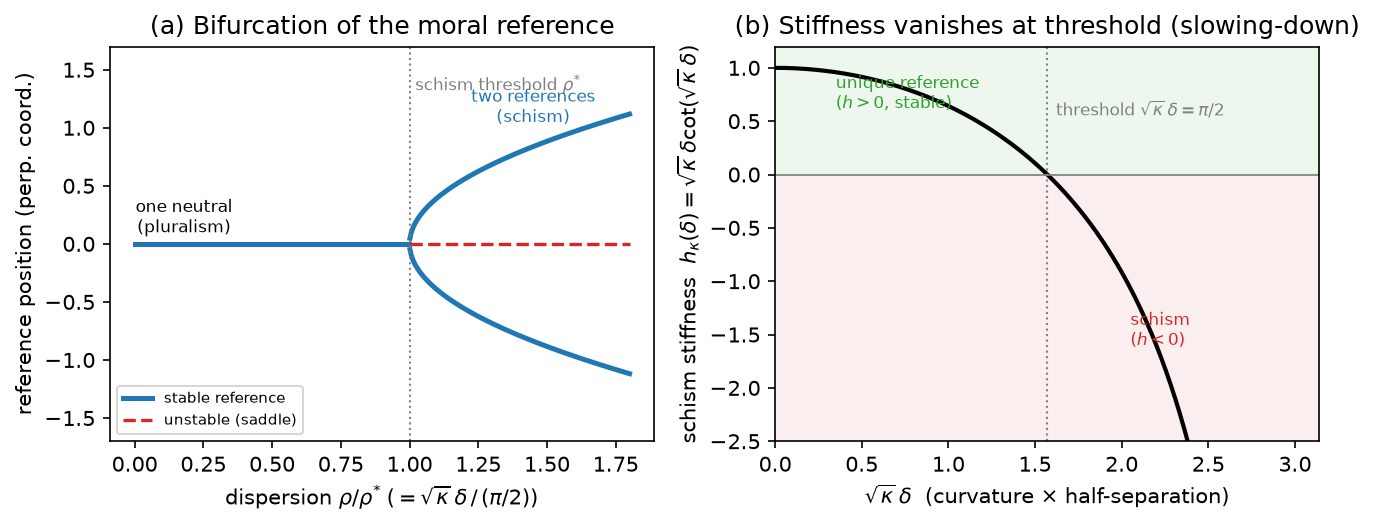
\includegraphics[keepaspectratio,alt={Schism as a bifurcation of the moral reference. (a) As dispersion \textbackslash rho crosses the curvature-set threshold \textbackslash rho\^{}\{*\}, the single floating neutral loses stability (dashed) and two competing references split off --- a pitchfork. (b) The exact schism stiffness h\_\textbackslash kappa(\textbackslash delta)=\textbackslash sqrt\{\textbackslash kappa\}\textbackslash,\textbackslash delta\textbackslash cot(\textbackslash sqrt\{\textbackslash kappa\}\textbackslash,\textbackslash delta) for the symmetric two-cluster sphere falls to zero at \textbackslash sqrt\{\textbackslash kappa\}\textbackslash,\textbackslash delta=\textbackslash pi/2; its vanishing is the critical slowing-down of §5.7.}]{figures/ert_bifurcation.png}}
\caption{\textbf{Schism as a bifurcation of the moral reference.} (a) As
dispersion \(\rho\) crosses the curvature-set threshold \(\rho^{*}\),
the single floating neutral loses stability (dashed) and two competing
references split off --- a pitchfork. (b) The exact schism stiffness
\(h_\kappa(\delta)=\sqrt{\kappa}\,\delta\cot(\sqrt{\kappa}\,\delta)\)
for the symmetric two-cluster sphere falls to zero at
\(\sqrt{\kappa}\,\delta=\pi/2\); its vanishing is the critical
slowing-down of §5.7.}
\end{figure}

\textbf{Why this is the right picture of schism.} Positive curvature in
value space is exactly the regime where the geodesic \emph{compromise}
between two positions is \textbf{worse than either pole} --- where
splitting the difference satisfies no one. That is the signature of
sacred or protected values, on which half-measures read as betrayal.
Negative or flat curvature is the regime of ordinary, tradeable values,
where intermediate positions are stable. ERT therefore predicts that
\textbf{schisms concentrate on the high-curvature (sacred/identity) axes
of the moral manifold and not on the tradeable ones} --- and it explains
schism \emph{without} either faction being in error (contra error
theory) and \emph{without} an external arbiter (no anchor): the two
post-schism communities are simply different stable basins of the same
Fréchet landscape, each internally coherent. The split is geometric, not
moral.

\subsubsection{5.7 Critical slowing-down: an early-warning
signal}\label{critical-slowing-down-an-early-warning-signal}

The threshold is not just a static fact; coupled to the reflexive
dynamics of §5.2--5.4 it becomes \emph{predictive}. As a population's
dispersion drifts toward \(\rho^{*}\) (driven by the reweighting term in
\((\star)\)), the orthogonal stiffness \(h_\kappa(\delta)\to 0\): the
reference's restoring curvature vanishes. This is the generic precursor
of a saddle-node/pitchfork bifurcation --- \textbf{critical
slowing-down} --- and it yields measurable early-warning signals
\emph{before} a schism actually occurs:

\begin{enumerate}
\def\labelenumi{\arabic{enumi}.}
\tightlist
\item
  \textbf{Rising recovery time} --- the aggregate reference relaxes ever
  more slowly after shocks (autocorrelation of \(R\) rises toward 1);
\item
  \textbf{Rising variance/volatility} of \(R\) under constant
  perturbation;
\item
  \textbf{Flattening} of the Fréchet landscape around \(R\) (the
  smallest Hessian eigenvalue trends to zero).
\end{enumerate}

Operationally, on longitudinal moral-survey or corpus time-series, a
community approaching schism should show its reference becoming
\emph{more volatile and slower to recover} in the run-up to the split
--- a prediction sharply distinct from ``the groups simply drifted
apart,'' and testable with the same instruments as §6. Schism, on this
account, is forecastable.

\textbf{Honest caveats.} The closed-form thresholds assume constant
curvature and the symmetric configuration; the real moral manifold is
stratified with variable curvature, so \(\rho^{*}\) is \emph{local} and
cut-locus structure matters (§5.8). The
curvature\(\,\leftrightarrow\,\)sacred-value correspondence is a
conjecture to be measured, not a result. And ``multiple Karcher means
exist'' is necessary, not sufficient, for an observed social schism ---
the dynamics must also carry sub-populations into the distinct basins.

\subsubsection{5.8 Open problems}\label{open-problems}

Existence, uniqueness, and stability of the self-referential equilibrium
on \(M\); the full bifurcation classification under joint \((v,w)\)
dynamics; conditions for Fréchet-mean uniqueness on the
\emph{stratified} moral manifold (cut-locus and curvature bounds beyond
{[}Afsari 2011{]}); and the empirical estimation of \(k_i, c_i, w_i\)
and the recovery of \((\star)\) from longitudinal moral-survey data. The
last is the bridge back to the corpus evidence of §6 and to the
falsification tests of §8.

\subsection{6. Evidence: why references
cluster}\label{evidence-why-references-cluster}

If \(R\) is endogenous, distinct societies are distinct load
configurations and should, in general, determine distinct references.
Why, then, the striking cross-cultural agreement on core norms?

ERT's answer is mechanical, not metaphysical: \textbf{human load
configurations cluster, so their neutrals cluster.} Shared embodiment,
shared social pressures, and shared dependence on cooperation make the
\(\{v_i, w_i\}\) of independent cultures similar enough that their
weighted Fréchet means fall near one another --- \emph{without} any
common external anchor pulling them there. Convergence is evidence of
\emph{similar loads}, not of a shared ground.

This reframes the empirical program of Geometric Ethics. Analysis of a
large cross-lingual normative corpus (≈109,000 passages across eleven
languages and roughly three millennia) {[}Bond 2026{]} finds that the
\emph{dimensional structure} of moral evaluation is stable across
languages and eras --- the same low-dimensional axes recur regardless of
framing. On ERT, that stability is the \textbf{phase structure} (the
dimensions along which loads can sit), and the cross-cultural agreement
on particular verdicts is the \textbf{clustering of neutrals} within it.
The program \emph{measures the neutral}; it does not legislate it.

One honest caveat carries over: the strongest decoding results are
measured \emph{through} a multilingual embedding model whose
language-agnostic representation may itself carry some of the apparent
universality. Until that confound is excluded, ``the axes are
invariant'' retains a deflationary reading --- which ERT can absorb (the
instrument would then be measuring a real but partly representational
structure) but should not hide.

\subsection{7. Relation to existing
positions}\label{relation-to-existing-positions}

ERT is not error theory: Mackie {[}1977{]} holds there are \emph{no}
moral facts, only systematic error; ERT holds there is a determinate
fact --- the location of \(R\) --- that simply lacks authority. It is
not quasi-realism (Blackburn {[}1998{]}): \(R\) is computed from real
loads, not projected from attitudes and then talked about \emph{as if}
real. It is closest in spirit to \textbf{constructivism} (Street
{[}2006{]}; Korsgaard {[}1996{]}) --- morality as constituted by valuers
rather than found --- but supplies what constructivism
characteristically lacks: an \emph{explicit, falsifiable construction}
(the weighted Fréchet mean) and a \emph{dynamics} (the control law). It
is compatible with naturalist programs (Railton {[}1986{]}; Boyd
{[}1988{]}) and with ``morality as cooperation'' (Curry et
al.~{[}2019{]}), which it can read as accounts of \emph{why the loads
sit where they do.} Its distinctive commitments are the two halves held
together: \textbf{realism about the reference, deflationism about
authority} --- a combination the standard taxonomy does not have a box
for, because the taxonomy presupposes the anchoring assumption ERT
denies.

\subsection{8. Falsifiability}\label{falsifiability}

In the Philosophy Engineering tradition, a metaethical claim earns its
keep by entailing testable predictions. ERT would be undermined if:

\begin{enumerate}
\def\labelenumi{\arabic{enumi}.}
\tightlist
\item
  \textbf{Reference indeterminacy.} Moral systems with stable, shared
  load configurations nonetheless exhibited \emph{no} determinate
  reference --- verdicts scattering with no computable center. (ERT
  predicts a determinate \(R\) wherever loads are well-defined.)
\item
  \textbf{Load-independence.} The reference failed to track the loads
  --- e.g., shifting valuations across a population left aggregate moral
  verdicts unchanged, or vice versa. (ERT predicts \(R\) moves with
  \(\{v_i, w_i\}\) as Millman/Fréchet prescribes.)
\item
  \textbf{Anchor signature.} Cross-cultural convergence persisted
  \emph{even where loads diverge} --- references coinciding despite
  dissimilar configurations --- which would be evidence of an external
  attractor (an anchor) after all, contra endogeneity.
\item
  \textbf{Dynamical mismatch.} Observed moral change failed to obey a
  feedback law of the stated form --- e.g., displacement from the
  current reference had no predictive relation to subsequent valuation
  shifts.
\item
  \textbf{Schism without curvature.} Communities fractured into stable,
  competing references \emph{independently of value-space curvature} ---
  splitting as readily on low-curvature (tradeable) axes as on
  high-curvature (sacred/identity) ones, or splitting while dispersion
  stayed well below the estimated threshold \(\rho^{*}\). (ERT predicts
  schism is confined to high-curvature axes and to \(\rho>\rho^{*}\);
  §5.6.) \emph{Concretely:} estimate the metric and curvature from the
  corpus/survey embedding, locate the high-\(\kappa\) axes, and test
  whether documented schisms (denominational splits, party realignments,
  professional-ethics fractures) concentrate there and cross the
  threshold --- not on the low-\(\kappa\) ones.
\item
  \textbf{Schism without warning.} Observed splits arrived as abrupt
  jumps with \emph{no} precursor --- no rise in the reference's recovery
  time or variance beforehand --- or those critical-slowing-down signals
  appeared just as often in communities that did \textbf{not} split.
  (ERT predicts a measurable slowing-down as \(\rho\to\rho^{*}\); §5.7.)
  \emph{Concretely:} on a moral time series, compute the lag-1
  autocorrelation and variance of the aggregate reference in a sliding
  window; ERT requires both to trend upward in the run-up to a schism
  and to be absent in matched non-splitting controls.
\end{enumerate}

These are demanding and, with population-scale moral measurement,
approachable. Tests 5--6 are the sharpest: they target the schism result
(§5.6--5.7), which has no scalar or flat-space analogue, so a clean
negative there would falsify ERT's distinctive content specifically ---
not merely some shared feature of structural metaethics.

\textbf{Preliminary results.} The accompanying artifact exercises these
tests rather than leaving them as promissory notes. The synthetic
confirmation is clean: the schism stiffness \(h_\kappa(\delta)\) matches
its closed form to four decimals and vanishes at
\(\sqrt\kappa\,\delta=\pi/2\), and the Fréchet reference bifurcates only
under positive curvature --- Proposition 2 holds numerically. A first
probe of Test 5 on real moral judgments (≈2,900 labelled AITA dilemmas)
was, by contrast, \textbf{inconclusive}: contestation showed no relation
to bimodality of the recovered moral-position axis (robust across two
encoders), but the test is underpowered --- the moral axis was only
weakly recoverable (AUC ≈ 0.60) on a heavily verdict-skewed corpus, and
the curvature half of Test 5 was not exercised. We report this as a null
the instrument cannot yet turn into a falsification; a decisive test
needs a polarized, vote-margin corpus and a direct curvature estimate.
In the Philosophy Engineering spirit, the failure is part of the record,
not hidden.

\textbf{Update --- the sacred-axis prediction is falsified.} The
decisive Test-5b run on Moral Machine AMCE preferences (177 agents: 176
LLMs plus one aggregate human, labelled 9-D --- no embedding, no AUC
ceiling) found that agent references \emph{do} cluster into \(\ge 2\)
basins (GMM BIC-optimal at 4 components; silhouette 0.36--0.40),
\textbf{but the multimodality concentrates on the
impartial/consequentialist axes} (number of lives, species), not the
\textbf{sacred/identity} ones (age, gender, status, fitness), which show
consensus --- Mann--Whitney sacred \(>\) impartial \(p=0.90\) (the wrong
direction). Combined with the GlobalOpinionQA null (\(n=26\)), ERT's
distinctive prediction --- that schism concentrates on
sacred/high-curvature axes (§5.6) --- has \textbf{zero confirmations and
is falsified on the best-powered instrument available}. What survives is
only the weaker claim that moral references bifurcate into camps, which
is ordinary opinion-dynamics clustering and not unique to ERT.
\emph{(Caveat: the exact per-country human AMCE matrix was unavailable
--- only an aggregate human column --- so the human-cultural version is
technically untested; but the mechanism failed on a strong, well-powered
proxy population on top of the GOQA null.)} ERT therefore rests on its
philosophical reframe (§§1--4) and its theorems (§5.2, §5.6),
\textbf{not} on this empirical signature; the schism result should be
read as a falsifiable conjecture that did not survive, reported in full
per the Philosophy Engineering commitment in §1.

\subsection{9. Limits and open problems}\label{limits-and-open-problems}

We close with what ERT does \emph{not} do. It \textbf{deflates}
bindingness; those who want morality to \emph{command} will find that
demand unmet --- by design, and they may reasonably regard this as
changing the subject rather than answering it. The \textbf{reflexive
dynamics} of §5 are stated, not solved; the existence, stability, and
uniqueness conditions of the self-referential equilibrium are open. The
\textbf{measurement} of \(R\) inherits the embedding-instrument confound
of §6. And there is a genuine \textbf{normativity-for-the-individual}
residue: ERT explains where the system's reference \emph{is} and why one
\emph{feels} strain, but an agent can still ask ``why should \emph{I}
reduce my displacement?'' --- to which ERT's only answer is the honest
one: \emph{no external authority requires you to; the consequences of
large displacement are simply real} --- the overvoltage does not ask
permission before it burns.

That answer will not satisfy everyone. But it is the answer the floating
neutral actually gives, and ERT's contribution is to give it precisely:
a moral reference that is real, computable, endogenous, consequential
--- and anchorless.

\begin{center}\rule{0.5\linewidth}{0.5pt}\end{center}

\subsection{References}\label{references}

\begin{itemize}
\tightlist
\item
  Afsari, B. (2011). Riemannian \(L^p\) center of mass: existence,
  uniqueness, and convexity. \emph{Proceedings of the American
  Mathematical Society}, 139(2), 655--673.
\item
  Blackburn, S. (1998). \emph{Ruling Passions: A Theory of Practical
  Reasoning}. Oxford University Press.
\item
  Bond, A. H. (2026). \emph{Geometric Ethics: A Foundational Theory of
  Moral Structure} (and the accompanying cross-lingual corpus analysis,
  ≈109,294 passages, 11 languages). Working paper / ErisML foundations.
\item
  Boyd, R. (1988). How to Be a Moral Realist. In G. Sayre-McCord (Ed.),
  \emph{Essays on Moral Realism} (pp.~181--228). Cornell University
  Press.
\item
  Curry, O. S., Mullins, D. A., \& Whitehouse, H. (2019). Is It Good to
  Cooperate? Testing the Theory of Morality-as-Cooperation in 60
  Societies. \emph{Current Anthropology}, 60(1), 47--69.
\item
  DeGroot, M. H. (1974). Reaching a Consensus. \emph{Journal of the
  American Statistical Association}, 69(345), 118--121.
\item
  Fréchet, M. (1948). Les éléments aléatoires de nature quelconque dans
  un espace distancié. \emph{Annales de l'Institut Henri Poincaré},
  10(4), 215--310.
\item
  Hegselmann, R., \& Krause, U. (2002). Opinion Dynamics and Bounded
  Confidence: Models, Analysis, and Simulation. \emph{Journal of
  Artificial Societies and Social Simulation}, 5(3).
\item
  Hume, D. (1739--40). \emph{A Treatise of Human Nature}. (Is/ought:
  Book III, Part I, §I.)
\item
  Karcher, H. (1977). Riemannian center of mass and mollifier smoothing.
  \emph{Communications on Pure and Applied Mathematics}, 30(5),
  509--541.
\item
  Korsgaard, C. M. (1996). \emph{The Sources of Normativity}. Cambridge
  University Press.
\item
  Mackie, J. L. (1977). \emph{Ethics: Inventing Right and Wrong}.
  Penguin.
\item
  Millman, J. (1940). A Useful Network Theorem. \emph{Proceedings of the
  IRE}, 28(9), 413--417.
\item
  Railton, P. (1986). Moral Realism. \emph{The Philosophical Review},
  95(2), 163--207.
\item
  Street, S. (2006). A Darwinian Dilemma for Realist Theories of Value.
  \emph{Philosophical Studies}, 127(1), 109--166.
\end{itemize}

\begin{center}\rule{0.5\linewidth}{0.5pt}\end{center}

\emph{Next steps: classify the self-referential equilibria on \(M\)
(§5.4, §5.8); design the load-independence and anchor-signature tests
(§8); add a schism-threshold / early-warning test to §8; reconcile the
reference \(R\) with the Geometric Ethics manifold formalism {[}Bond
2026{]}; and attempt empirical recovery of \((\star)\) from longitudinal
moral-survey data.}

\end{document}
